\documentclass[12pt,a4paper]{article}
\usepackage[utf8]{inputenc}
\usepackage[T5]{fontenc}
\usepackage[vietnamese]{babel}
\usepackage{geometry}
\usepackage{longtable}
\usepackage{booktabs}
\usepackage{amsmath}
\usepackage[hidelinks,unicode]{hyperref}
\usepackage[table]{xcolor}
\usepackage{lmodern}
\usepackage{enumitem}
\usepackage{caption}
\usepackage{tikz}
\usepackage{graphicx}
\usepackage{indentfirst}
\usepackage{float}
\usepackage{fancyhdr}
\usepackage{titlesec}
\usepackage{tabularx}
\usetikzlibrary{shapes, arrows, positioning, fit, calc, mindmap, trees, shadows}

\geometry{a4paper, margin=1in, top=1.2in}

\pagestyle{fancy}
\fancyhf{}
\fancyhead[L]{\footnotesize Tính toán khoa học thần kinh} % Đổi tiêu đề header trái
\fancyhead[R]{\footnotesize UET - VNU}
\fancyfoot[C]{\thepage}
\renewcommand{\headrulewidth}{0.4pt}
\renewcommand{\footrulewidth}{0.4pt}

% Định dạng section (Giữ nguyên)
\titleformat{\section}
  {\normalfont\Large\bfseries}{\thesection}{1em}{}
\titleformat{\subsection}
  {\normalfont\large\bfseries}{\thesubsection}{1em}{}
\titleformat{\subsubsection}
  {\normalfont\normalsize\bfseries}{\thesubsubsection}{1em}{}

\begin{document}

% =============== TRANG BÌA ===============
\begin{titlepage}
    % --- VẼ KHUNG VIỀN ---
    \begin{tikzpicture}[overlay,remember picture]
        \draw [line width=3pt]
            ($ (current page.north west) + (2.5cm,-2.0cm) $)
            rectangle
            ($ (current page.south east) + (-1.5cm,2.0cm) $);
        \draw [line width=1pt]
            ($ (current page.north west) + (2.65cm,-2.15cm) $)
            rectangle
            ($ (current page.south east) + (-1.65cm,2.15cm) $);
    \end{tikzpicture}

    \centering

    % --- PHẦN 1: HEADER TRƯỜNG & LOGO ---
    \vspace*{0.2cm}
    {\fontsize{14}{16}\selectfont \textbf{ĐẠI HỌC QUỐC GIA HÀ NỘI}}\\[0.2cm]
    {\fontsize{15}{18}\selectfont \textbf{TRƯỜNG ĐẠI HỌC CÔNG NGHỆ}}\\[0.2cm]
    \rule{8cm}{0.8pt}

    \vspace{1.2cm}
    
\includegraphics[width=3.3cm]{uet.png}

    \vspace{1.3cm}

    % --- PHẦN 2: TIÊU ĐỀ ---
    {\fontsize{18}{22}\selectfont \textbf{BÁO CÁO HỌC PHẦN DỰ ÁN}}\\[1.1cm]

    {\fontsize{24}{28}\selectfont \textbf{ĐỀ TÀI}}\\[0.5cm]

    {\fontsize{22}{26}\selectfont
    \textbf{HỆ THỐNG HYBRID - LLM}}\\[0.2cm]
    {\fontsize{22}{26}\selectfont
    \textbf{GIẢI TOÁN KẾT HỢP CHẤM BÀI}}\\[0.2cm]
    {\fontsize{22}{26}\selectfont}

    \vspace{2.4cm}

    % --- PHẦN 3: BẢNG TÊN ---
    \begin{center}
    \large
    \renewcommand{\arraystretch}{1.45}

    \begin{tabular}{l l r}
    \textbf{Giảng viên hướng dẫn:}
    & PGS.TS Nguyễn Việt Hà & \\
    &  ThS. Nguyễn Thị Thùy Linh & \\[0.3cm]

    \textbf{Nhóm sinh viên thực hiện:}
    & Ngô Đình Linh
    & 23020394 \\

    &
    Nguyễn Trần Huy
    & 23020378 \\

    &
    Nguyễn Đức Huy
    & 23020376 \\
    \end{tabular}
    \end{center}

    \vspace{1.0cm}

    % --- PHẦN 4: NGÀY THÁNG ---
    {\large \textbf{Hà Nội, tháng 6 năm 2026}}

\end{titlepage}
% =============== PHẦN CHẤN ĐIỂM VÀ NHẬN XÉT ===============

% =============== Ý KIẾN ĐÁNH GIÁ ===============
\newpage
\thispagestyle{empty}

\begin{center}
    {\Large \textbf{Ý KIẾN ĐÁNH GIÁ}}
\end{center}

\vspace{0.8cm}

\noindent
\textbf{Ý kiến đánh giá:}

\vspace{0.5cm}

\noindent
\makebox[\textwidth]{\dotfill}\\[0.6cm]
\makebox[\textwidth]{\dotfill}\\[0.6cm]
\makebox[\textwidth]{\dotfill}\\[0.6cm]
\makebox[\textwidth]{\dotfill}\\[0.6cm]
\makebox[\textwidth]{\dotfill}\\[0.6cm]
\makebox[\textwidth]{\dotfill}\\[0.6cm]
\makebox[\textwidth]{\dotfill}\\[0.6cm]
\makebox[\textwidth]{\dotfill}\\[0.6cm]
\makebox[\textwidth]{\dotfill}\\[1cm]

\noindent
\textbf{Điểm số:} \dotfill \hspace{1cm}
\textbf{Điểm chữ:} \dotfill

\vspace{1.2cm}

\begin{flushright}
    Hà Nội, ngày \dots, tháng \dots, năm 20\dots
\end{flushright}

\vspace{1cm}

\begin{flushright}
    \textbf{Giảng viên đánh giá}\\
    \textit{(Ký, ghi rõ họ tên)}
\end{flushright}


% =============== LỜI CẢM ƠN ===============
\newpage
\thispagestyle{empty}

\begin{center}
    {\Large \textbf{LỜI CẢM ƠN}}
\end{center}

\vspace{0.8cm}




Lời đầu tiên, chúng em xin được gửi lời cảm ơn chân thành nhất đến thầy Nguyễn Việt Hà và cô Nguyễn Thị Thùy Linh. 
Trong quá trình học tập và thực hiện học phần Dự án, chúng em đã nhận được sự quan tâm, 
hướng dẫn tận tình và những góp ý quý báu từ thầy cô.

Nhờ sự định hướng của cô, nhóm chúng em có thêm cơ hội tìm hiểu, nghiên cứu và triển khai đề tài 
\textbf{``Hệ thống HYBRID-LLM giải toán kết hợp chấm bài''}. 
Đề tài giúp chúng em vận dụng các kiến thức đã học vào việc xây dựng một hệ thống hỗ trợ chấm bài và gia sư học sinh trong quá trình giải toán, 
không chỉ đưa ra đáp án cuối cùng mà còn cung cấp các gợi ý phù hợp nhằm giúp người học hiểu rõ hơn phương pháp giải.

Trong dự án này, nhóm chúng em tập trung xây dựng một hệ thống có khả năng tiếp nhận đề bài hoặc lời giải của học sinh thông qua văn bản hoặc hình ảnh. Đối với dữ liệu hình ảnh, hệ thống sử dụng OCR để trích xuất nội dung bài toán, từ đó hỗ trợ quá trình xử lý đầu vào một cách trực quan và thuận tiện hơn. Bên cạnh đó, nhóm triển khai pipeline gồm các bước \textit{formalize}, \textit{solve} và \textit{verify} cho các bài toán dạng GSM8K. Cụ thể, hệ thống sử dụng mô hình ngôn ngữ lớn để chuyển đổi đề bài và lời giải của học sinh thành các file YAML có cấu trúc, sau đó kiểm tra các quan hệ tính toán và so sánh lời giải chuẩn với lời giải của học sinh. Trong quá trình thực hiện báo cáo và xây dựng hệ thống, do kiến thức và kinh nghiệm của nhóm còn hạn chế, bài làm chắc chắn khó tránh khỏi những thiếu sót. Chúng em kính mong nhận được những nhận xét và góp ý của cô để báo cáo cũng như sản phẩm của nhóm được hoàn thiện hơn. 
Chúng em xin chân thành cảm ơn!



% =============== TỔNG QUAN ===============
% \newpage
% \thispagestyle{empty}

% \begin{center}
%     {\Large \textbf{TỔNG QUAN}}
% \end{center}

% \vspace{0.8cm}

% Báo cáo này trình bày quá trình nghiên cứu và xây dựng đề tài 
% \textbf{``Hệ thống giải toán kết hợp đưa ra gợi ý cho học sinh''}. 
% Mục tiêu của đề tài là xây dựng một hệ thống hỗ trợ học sinh trong quá trình học tập môn Toán, 
% giúp người học không chỉ nhận được lời giải cho bài toán mà còn có thể tiếp cận từng bước thông qua các gợi ý phù hợp.

% Trong thực tế, nhiều học sinh khi gặp một bài toán khó thường có xu hướng tìm ngay đáp án cuối cùng. 
% Tuy nhiên, cách học này có thể khiến học sinh chưa hiểu đầy đủ bản chất của bài toán và phương pháp giải. 
% Vì vậy, hệ thống được định hướng theo hướng hỗ trợ học tập, trong đó việc đưa ra gợi ý từng bước đóng vai trò quan trọng. 
% Các gợi ý này giúp học sinh suy nghĩ, tự hoàn thiện lời giải và rèn luyện khả năng tư duy thay vì chỉ phụ thuộc vào đáp án có sẵn.

% Về mặt chức năng, hệ thống hướng đến việc tiếp nhận đề bài toán từ người dùng, phân tích nội dung bài toán, 
% sau đó sinh ra lời giải hoặc các gợi ý theo từng mức độ. 
% Tùy theo trạng thái của người học, hệ thống có thể đưa ra gợi ý ban đầu, gợi ý phương pháp, hoặc hướng dẫn chi tiết hơn để hỗ trợ quá trình giải bài.

% Báo cáo được tổ chức thành các phần chính, bao gồm giới thiệu bài toán, cơ sở lý thuyết, phương pháp xây dựng hệ thống, 
% quá trình thực nghiệm, đánh giá kết quả và kết luận. 
% Thông qua đề tài này, nhóm mong muốn xây dựng một sản phẩm có tính ứng dụng trong giáo dục, 
% đồng thời củng cố kiến thức về xử lý ngôn ngữ tự nhiên, mô hình ngôn ngữ và thiết kế hệ thống hỗ trợ học tập.


% =============== MỚI BẮT ĐẦU NỘI DUNG ===============
\newpage
\fancyhead[L]{Mục lục} 
\tableofcontents
\listoffigures
\newpage


\fancyhead[L]{\nouppercase{\leftmark}} 

% =========================================================
% SECTION 1: GIỚI THIỆU
% =========================================================
\section{Giới thiệu}

\subsection{Bối cảnh}
Hiện nay, việc chấm và phân tích lời giải toán nhiều bước vẫn là một điểm nghẽn trong dạy học và các hệ thống trí tuệ nhân tạo giáo dục. Với các bài toán yêu cầu lập luận theo từng bước, việc chỉ kiểm tra đáp án cuối cùng là chưa đủ, vì học sinh có thể sai ở nhiều vị trí khác nhau như đọc sai dữ kiện, chọn sai phép tính, nhầm đơn vị hoặc tính toán sai kết quả trung gian. Trong thực tế, giáo viên thường phải phân tích thủ công quá trình làm bài, trong khi nhiều hệ thống chấm tự động đơn giản chưa đánh giá được đầy đủ chuỗi lập luận của học sinh.

Các mô hình ngôn ngữ lớn có thể hỗ trợ đọc hiểu đề bài và lời giải, nhưng nếu sử dụng trực tiếp như một bộ chấm tự do, hệ thống dễ gặp các vấn đề như ảo giác, suy luận không nhất quán hoặc đưa ra nhận xét thiếu căn cứ. Vì vậy, đề tài hướng tới xây dựng một hệ thống chấm lời giải toán tự động theo hướng có cấu trúc, trong đó lời giải và bài làm được formalize thành các thực thể, biểu thức và bước suy luận có thể kiểm tra được.

Mục tiêu chính của hệ thống là hỗ trợ giáo viên và các hệ thống chấm tự động trong việc đánh giá quá trình làm bài của học sinh một cách chi tiết hơn, đồng thời tạo ra các thành phần kiểm tra có cấu trúc có thể đóng vai trò như validator cho việc đánh giá hoặc huấn luyện mô hình AI giải toán. Ngoài nhánh chấm bài dựa trên bài mẫu, hệ thống còn có thể sinh lời giải tham chiếu để hỗ trợ học sinh trong vai trò gia sư khi cần thiết.

\subsection{Mục tiêu}

Dự án được thiết kế gồm hai nhánh xử lý chính: nhánh so sánh lời giải và nhánh sinh lời giải. Cả hai nhánh đều sử dụng các thực thể đã được formalize từ đề bài làm nền tảng chung. Trong nhánh so sánh, hệ thống tiếp tục formalize bài mẫu của giáo viên và bài làm của học sinh, sau đó đối chiếu hai lời giải để hỗ trợ chấm bài và phát hiện lỗi. Trong nhánh sinh lời giải, hệ thống tạo lời giải tham chiếu từ đề bài khi chưa có bài mẫu, rồi sử dụng lời giải này làm cơ sở cho việc so sánh và hỗ trợ học sinh.

Để hiện thực hóa định hướng trên, hệ thống tập trung vào các mục tiêu chính sau:

\begin{itemize}[leftmargin=*]
\item \textbf{Formalize đề bài, bài mẫu và bài làm của học sinh:}
chuyển các nội dung đầu vào thành danh sách thực thể và các bước có cấu trúc, bao gồm dữ kiện, đại lượng cần tìm, biểu thức, kết quả trung gian và đơn vị.

\item \textbf{Xây dựng nhánh so sánh lời giải:}
ánh xạ các thực thể và bước tính trong bài làm của học sinh với bài mẫu hoặc lời giải tham chiếu, dựa trên giá trị, đơn vị, vai trò và quan hệ biểu thức giữa các đại lượng.

\item \textbf{Phát hiện lỗi ở mức từng bước:}
xác định vị trí bắt đầu sai lệch và phân loại các lỗi như dùng sai dữ kiện, chọn sai phép toán, tính toán nhầm, thiếu bước, sai đơn vị hoặc tạo ra đại lượng trung gian không phù hợp.

\item \textbf{Xây dựng nhánh sinh lời giải phục vụ gia sư:}
trong trường hợp không có bài mẫu, hệ thống lập kế hoạch giải từ các thực thể đã formalize của đề bài, tạo lời giải tham chiếu và kiểm tra tính hợp lệ của các bước tính toán.

\item \textbf{Tạo phản hồi dựa trên kết quả phân tích:}
cung cấp nhận xét cụ thể cho giáo viên hoặc học sinh, tập trung vào bước sai và nguyên nhân sai thay vì chỉ thông báo đáp án đúng hoặc sai.

\item \textbf{Đánh giá hệ thống trên 200 bài GSM8K:}
thử nghiệm khả năng formalize, sinh lời giải, ánh xạ lời giải và phát hiện lỗi trên các bài toán đố nhiều bước, trong cả hai kịch bản có bài mẫu và không có bài mẫu.

\item \textbf{Mở rộng khả năng tiếp nhận bài làm thực tế:}
tích hợp OCR trong giai đoạn tiếp theo để xử lý ảnh chụp đề bài, bài mẫu và lời giải của học sinh trước khi đưa vào quy trình formalize, so sánh và sinh lời giải.

\end{itemize}





\subsection{Tổng quan giải pháp}
Giải pháp tổng thể được tổ chức thành hai nhánh chính như minh họa trong
Hình~\ref{fig:project-overview}: khối xử lý AI (\textit{AI Engine})
và khối giao diện kết hợp nhận dạng văn bản từ ảnh (\textit{UI + OCR}).

\begin{figure}[htbp]
    \centering
    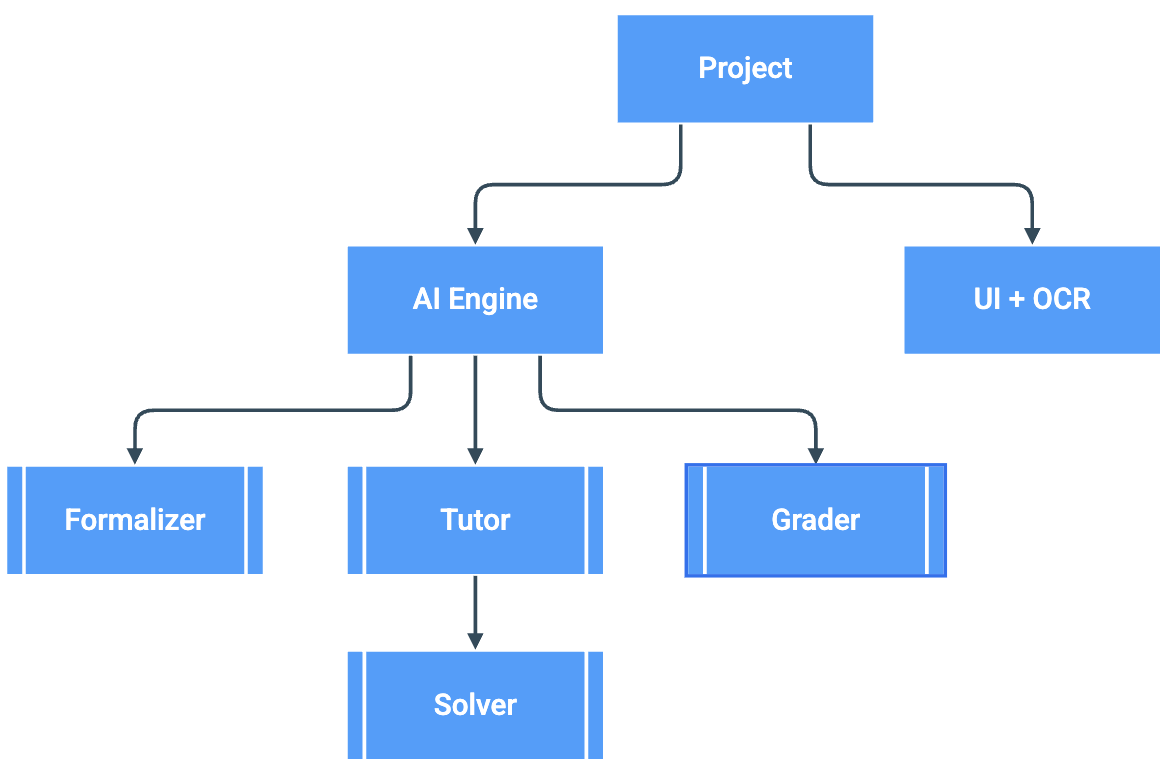
\includegraphics[width=0.9\linewidth]{structure.png}
    \caption{Tổng quan các thành phần của dự án}
    \label{fig:project-overview}
\end{figure}

Khối \textit{UI + OCR} đóng vai trò tiếp nhận dữ liệu từ người dùng.Học sinh có thể cung cấp ảnh chụp đề bài hoặc bài làm thay
vì phải nhập lại toàn bộ nội dung. Thành phần OCR chuyển dữ liệu ảnh thành văn
bản để khối AI tiếp tục phân tích.

\textit{AI Engine} là phần lõi của hệ thống, đảm nhiệm việc xử lý đề bài, lời giải tham chiếu và bài làm của học sinh dưới dạng có cấu trúc. Thay vì để mô hình ngôn ngữ trực tiếp đưa ra kết luận đúng sai, hệ thống chia quá trình xử lý thành các bước rõ ràng: formalize dữ liệu đầu vào, sinh hoặc tiếp nhận lời giải chuẩn, ánh xạ lời giải của học sinh với lời giải chuẩn và chẩn đoán lỗi sai.

Bên trong \textit{AI Engine}, dự án được tổ chức thành ba nhóm chức năng chính. Nhóm \textit{Formalizer} chuyển đề bài, bài mẫu của giáo viên và bài làm của học sinh từ ngôn ngữ tự nhiên sang các thực thể, biểu thức và bước lập luận có cấu trúc. Nhóm \textit{Solver} được sử dụng trong trường hợp chưa có bài mẫu, có nhiệm vụ tạo lời giải tham chiếu từ đề bài và kiểm tra tính hợp lệ của các bước tính toán. Nhóm \textit{Grader} thực hiện ánh xạ giữa lời giải học sinh với bài mẫu hoặc lời giải tham chiếu, từ đó xác định vị trí sai lệch và phân loại nguyên nhân lỗi.

Dự án sử dụng cách tiếp cận hybrid giữa mô hình ngôn ngữ lớn (Large Language Model -- LLM) và xử lý ký hiệu bằng Python. LLM được dùng để hỗ trợ đọc hiểu các cách diễn đạt đa dạng trong đề bài và lời giải, trong khi các bước kiểm tra quan trọng như thực thi biểu thức, kiểm tra đơn vị, ánh xạ thực thể và truy vết lỗi được thực hiện trên biểu diễn có cấu trúc. Cách kết hợp này giúp hệ thống tận dụng khả năng xử lý ngôn ngữ của LLM nhưng vẫn giảm phụ thuộc vào các nhận định tự do dễ gây ảo giác.

Trong phạm vi mã nguồn hiện tại, dự án tập trung triển khai phần lõi của \textit{AI Engine}, bao gồm formalize dữ liệu, sinh lời giải tham chiếu, kiểm tra lời giải và chẩn đoán lỗi trong bài làm của học sinh. Khối \textit{UI + OCR} và cơ chế tạo phản hồi mang tính sư phạm sẽ được phát triển ở các giai đoạn tiếp theo, nhằm giúp hệ thống tiếp nhận bài làm thực tế và đưa ra gợi ý phù hợp hơn cho học sinh.


% =========================================================
% SECTION 2: KIẾN TRÚC HỆ THỐNG
% =========================================================
\section{Kiến trúc hệ thống}

\subsection{Kiến trúc tổng thể}

Luồng hoạt động chi tiết của hệ thống được trình bày trong Hình~\ref{fig:detailed-system-flow}. Hệ thống được tổ chức xung quanh phần lõi \textit{AI Engine}, trong đó các bước xử lý chính gồm formalize dữ liệu đầu vào, sinh lời giải tham chiếu khi cần thiết và so sánh lời giải để chẩn đoán lỗi.

Cụ thể, hệ thống có hai nhánh xử lý chính. Nhánh \textit{Grader} được sử dụng khi đã có bài mẫu hoặc lời giải chuẩn do giáo viên cung cấp. Khi đó, hệ thống formalize đề bài, bài mẫu và bài làm của học sinh, sau đó ánh xạ các bước tương ứng để phát hiện sai lệch trong quá trình lập luận. Nhánh \textit{Solver} được sử dụng trong trường hợp chưa có bài mẫu; hệ thống sẽ sinh lời giải tham chiếu từ đề bài, kiểm tra tính hợp lệ của lời giải này, rồi dùng nó làm cơ sở cho quá trình so sánh và phản hồi.

Cách tổ chức này cho phép hệ thống hoạt động trong cả hai bối cảnh: hỗ trợ giáo viên chấm bài dựa trên lời giải mẫu có sẵn, và hỗ trợ học sinh theo vai trò gia sư khi cần tự sinh lời giải tham chiếu. Các phản hồi hoặc gợi ý cho học sinh được xây dựng dựa trên kết quả chẩn đoán lỗi, thay vì chỉ dựa trên đáp án cuối cùng.


\begin{figure}[htbp]
    \centering
    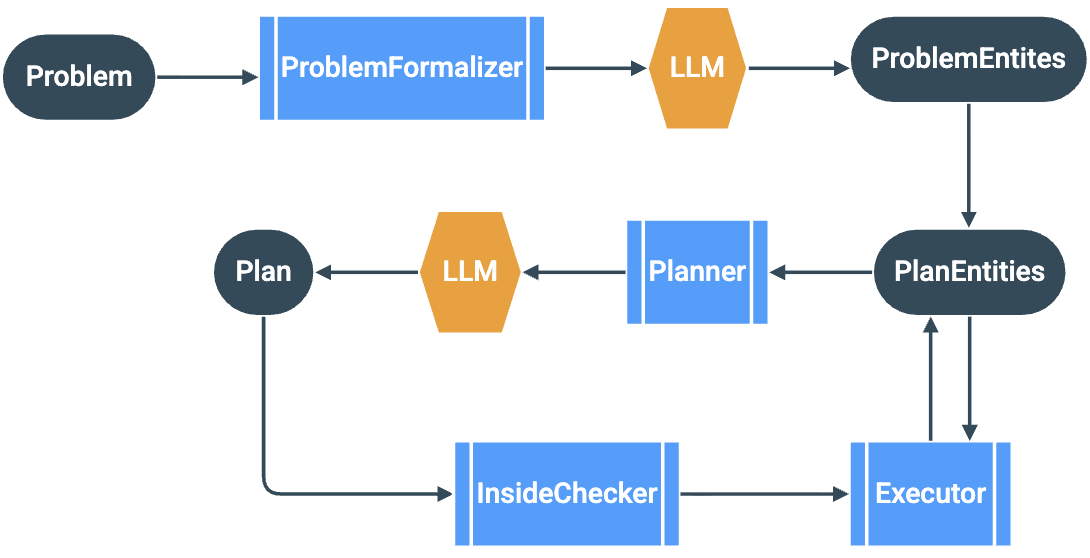
\includegraphics[width=\linewidth]{Solver.png}
    \caption{Luồng hoạt động chi tiết của hệ thống giải toán}
    \label{fig:detailed-system-flow}
\end{figure}

\begin{figure}[htbp]
    \centering
    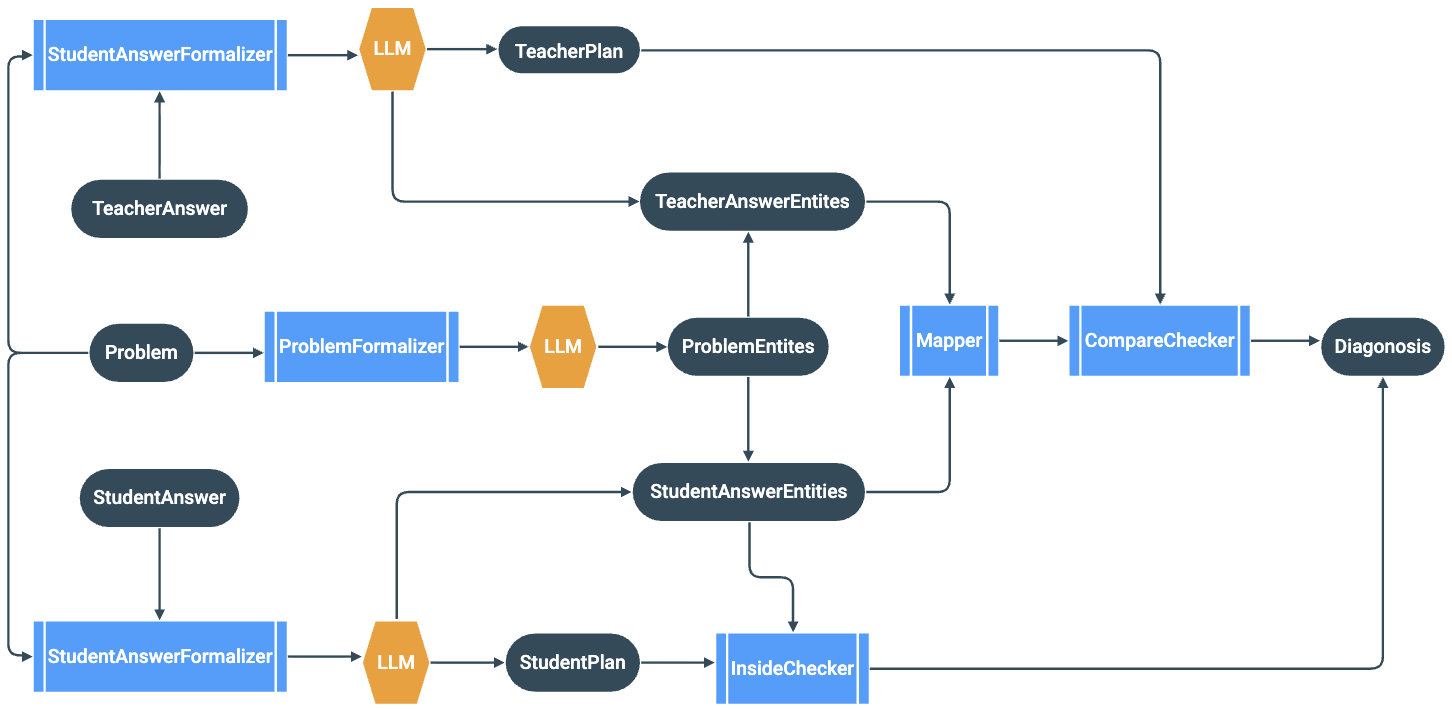
\includegraphics[width=\linewidth]{Grader.png}
    \caption{Luồng hoạt động chi tiết của hệ thống chấm điểm}
    \label{fig:detailed-system-flow}
\end{figure}

Ở giai đoạn hiện tại, đầu vào của hệ thống là văn bản được nhập trực tiếp.
Trong kiến trúc hoàn chỉnh, nội dung này cũng có thể được trích xuất từ ảnh
chụp thông qua OCR. Sau khi tiếp nhận dữ liệu, hệ thống tạo một lời giải tham
chiếu, phân tích cách làm của học sinh và lần lượt kiểm tra các bằng chứng thu
được. Kết quả cuối cùng không dừng lại ở việc xác định đúng hoặc sai, mà còn
phải đủ rõ để làm cơ sở cho một gợi ý có ích đối với người học.


\subsection{Các khối chức năng chính trong AI Engine}

Bên trong \textit{AI Engine}, hệ thống được chia thành nhiều khối chức năng nhỏ. Mỗi khối đảm nhiệm một vai trò riêng trong quá trình chuyển đổi dữ liệu, sinh lời giải hoặc chấm lời giải. Cách chia nhỏ này giúp hệ thống hạn chế việc để LLM trực tiếp đưa ra kết luận cuối cùng, đồng thời tạo điều kiện để kiểm tra và truy vết lỗi ở từng bước.

\subsubsection{ProblemFormalizer}

\textit{ProblemFormalizer} nhận đầu vào là đề bài ở dạng ngôn ngữ tự nhiên và chuyển đổi nội dung này thành danh sách các thực thể bài toán, gọi là \textit{ProblemEntities}. Các thực thể này biểu diễn những dữ kiện được cho trực tiếp trong đề bài, đơn vị đi kèm, ngữ cảnh sử dụng và đại lượng cần tìm. Đây là lớp biểu diễn nền tảng được dùng chung cho cả nhánh sinh lời giải và nhánh chấm bài.

\subsubsection{Planner}

\textit{Planner} được sử dụng trong nhánh sinh lời giải tham chiếu. Từ đề bài và các thực thể đã được chuẩn hóa, khối này yêu cầu LLM tạo ra một kế hoạch giải gồm các bước tính toán tuần tự. Kết quả của khối này là \textit{Plan}, trong đó mỗi bước mô tả biểu thức cần tính, kết quả mong đợi và đơn vị của đại lượng được tạo ra.

\subsubsection{Executor}

\textit{Executor} thực thi các biểu thức trong \textit{Plan} dựa trên các thực thể hiện có. Sau mỗi bước, hệ thống cập nhật thêm các đại lượng trung gian vào \textit{PlanEntities}. Vai trò của khối này là biến kế hoạch giải từ dạng mô tả thành các phép tính có thể kiểm tra được, qua đó giúp phát hiện những sai lệch về biểu thức, kết quả hoặc đơn vị.

\subsubsection{InsideChecker}

\textit{InsideChecker} kiểm tra tính hợp lệ nội bộ của lời giải hoặc bài làm đã được formalize. Trong nhánh sinh lời giải, khối này kiểm tra xem lời giải tham chiếu có sử dụng đúng dữ kiện, tạo ra đúng đại lượng cần tìm và có chuỗi suy luận hợp lệ hay không. Trong nhánh chấm bài, khối này cũng có thể được dùng để phát hiện các lỗi nội tại trong lời giải của học sinh trước khi so sánh với bài mẫu.

\subsubsection{StudentAnswerFormalizer}

\textit{StudentAnswerFormalizer} nhận đầu vào là bài làm của học sinh và chuyển bài làm này thành hai thành phần có cấu trúc: \textit{StudentPlan} và \textit{StudentAnswerEntities}. \textit{StudentPlan} biểu diễn các bước lập luận hoặc phép tính mà học sinh đã trình bày, còn \textit{StudentAnswerEntities} lưu các đại lượng xuất hiện trong bài làm. Nhờ đó, hệ thống có thể phân tích quá trình làm bài thay vì chỉ xét đáp án cuối cùng.

\subsubsection{TeacherAnswerFormalizer}

\textit{TeacherAnswerFormalizer} được sử dụng khi giáo viên cung cấp bài mẫu. Khối này chuyển lời giải chuẩn thành \textit{TeacherPlan} và \textit{TeacherAnswerEntities}. Các thành phần này đóng vai trò làm chuẩn so sánh trong nhánh chấm bài. Khi không có bài mẫu, vai trò của lời giải chuẩn có thể được thay thế bằng \textit{Plan} và \textit{PlanEntities} do nhánh sinh lời giải tạo ra.

\subsubsection{Mapper}

\textit{Mapper} thực hiện ánh xạ giữa các thực thể và bước giải trong bài làm của học sinh với các thành phần tương ứng trong bài mẫu hoặc lời giải tham chiếu. Việc ánh xạ không chỉ dựa trên tên gọi, mà còn dựa trên giá trị, đơn vị, vai trò của đại lượng và quan hệ biểu thức giữa các bước. Đây là bước trung gian quan trọng để hệ thống xác định học sinh đang đi đúng ở đâu và bắt đầu sai lệch từ bước nào.

\subsubsection{CompareChecker}

\textit{CompareChecker} sử dụng kết quả ánh xạ từ \textit{Mapper} để so sánh lời giải của học sinh với lời giải chuẩn. Khối này phát hiện các dạng sai lệch như dùng sai dữ kiện, sai phép toán, sai kết quả trung gian, thiếu bước hoặc sai đơn vị. Đầu ra của khối này là \textit{Diagnosis}, tức bản chẩn đoán mô tả vị trí lỗi, nguyên nhân lỗi và các thông tin liên quan đến bước sai.

\subsubsection{Diagnosis}

\textit{Diagnosis} là kết quả cuối cùng của nhánh chấm bài. Thành phần này không chỉ cho biết bài làm đúng hay sai, mà còn mô tả lỗi xuất hiện ở bước nào và vì sao lỗi đó xảy ra. Kết quả chẩn đoán có thể được sử dụng để hỗ trợ giáo viên trong quá trình chấm bài, hoặc làm cơ sở để hệ thống tạo phản hồi, gợi ý cho học sinh trong chế độ gia sư.

% =========================================================
% SECTION 3: CHI TIẾT KỸ THUẬT
% =========================================================
\section{Chi tiết kỹ thuật}

\subsection{Mục tiêu thiết kế}

Thiết kế ban đầu trong \texttt{Docs/Prompt.pdf} định hướng hệ thống theo dạng
hybrid: LLM chịu trách nhiệm đọc hiểu ngôn ngữ tự nhiên, còn Python chịu trách
nhiệm thực thi biểu thức, cập nhật entity, ánh xạ lời giải và kiểm tra lỗi. Vì
vậy, hệ thống không để LLM trực tiếp đưa ra kết luận cuối cùng ở mọi bước, mà
buộc dữ liệu phải đi qua các file trung gian có cấu trúc.

Phần lõi hiện tại có hai luồng chính. Luồng \textit{Tutor} tự sinh lời giải
tham chiếu từ đề bài thông qua \texttt{ProblemFormalizer},
\texttt{Planner} và \texttt{Executor}. Luồng \textit{Grader} chấm bài dựa trên
lời giải giáo viên bằng cách formalize cả bài làm học sinh và lời giải giáo
viên, sau đó chạy \texttt{InsideChecker}, \texttt{Mapper},
\texttt{CompareChecker} và khi cần thì dùng \texttt{LLMChecker} làm fallback.

\subsection{Biểu diễn dữ liệu trung gian}

Đầu vào ban đầu là văn bản trong \texttt{Input/Problem.txt},
\texttt{Input/StudentAnswer.txt} và \texttt{Input/TeacherAnswer.txt}. Sau khi
formalize, hệ thống tạo các file YAML trong thư mục \texttt{Output/}. Những file
này vừa là dữ liệu nội bộ cho pipeline, vừa là bằng chứng để người phát triển có
thể debug từng stage.

\subsubsection{Thực thể bài toán}

\texttt{ProblemEntities.yaml} chứa các đại lượng được cho trực tiếp trong đề
bài và đúng một target cần tìm. Theo prompt gốc, entity có bốn trường chính:
\texttt{value}, \texttt{unit}, \texttt{location} và \texttt{grand\_unit}. Code
hiện tại mở rộng thêm trường \texttt{source} để lưu bằng chứng văn bản, đồng
thời có thể thêm helper constant như \texttt{unit\_conversion\_*} để các bước
sau không phải viết số literal trong \texttt{expr}.

\begin{table}[H]
\centering
\small
\renewcommand{\arraystretch}{1.35}
\begin{tabularx}{\linewidth}{@{}p{0.30\linewidth}p{0.12\linewidth}p{0.13\linewidth}X@{}}
\toprule
\textbf{Entity} & \textbf{value} & \textbf{location} & \textbf{Ý nghĩa} \\
\midrule
\texttt{first\_child\_height} & 6 feet & input & Chiều cao đứa con thứ nhất, lấy trực tiếp từ đề bài. \\
\begin{tabular}[t]{@{}l@{}}\texttt{second\_child\_height}\\\texttt{\_taller\_than\_first}\end{tabular} & 2 inches & input & Độ cao hơn của đứa con thứ hai so với đứa thứ nhất. \\
\begin{tabular}[t]{@{}l@{}}\texttt{third\_child\_height}\\\texttt{\_shorter\_than\_second}\end{tabular} & 5 inches & input & Độ thấp hơn của đứa con thứ ba so với đứa thứ hai. \\
\texttt{fourth\_child\_height} & null & target & Đại lượng cần tìm: chiều cao đứa con thứ tư theo inches. \\
\begin{tabular}[t]{@{}l@{}}\texttt{unit\_conversion}\\\texttt{\_inches\_per\_foot}\end{tabular} & 12 & input & Hằng số đổi đơn vị do backbone thêm để biểu thức vẫn dùng biến. \\
\bottomrule
\end{tabularx}
\caption{Ví dụ rút gọn từ \texttt{Output/ProblemEntities.yaml}}
\label{tab:problem-entities-current-example}
\end{table}

Điểm quan trọng là \texttt{ProblemEntities.yaml} không được chứa kết quả trung
gian cần phải tính mới biết. Ví dụ, chiều cao đứa con thứ hai theo inches không
được tạo sẵn trong bước formalize đề bài; nó phải được tạo sau ở bước plan hoặc
answer formalizer.

\subsubsection{Plan, reported expression và formalized expression}

Mỗi lời giải được biểu diễn bằng các bước trong \texttt{Plan.yaml},
\texttt{StudentPlan.yaml} hoặc \texttt{TeacherPlan.yaml}. Một bước có hai lớp
biểu thức:

\begin{itemize}[leftmargin=*]
    \item \texttt{expr}: quan hệ symbolic bằng tên entity, ví dụ
    \texttt{first\_child\_height * unit\_conversion\_inches\_per\_foot}.
    \item \texttt{reported\_expr}: phép tính số thật được lời giải trình bày,
    ví dụ \texttt{6 * 12 = 72}.
\end{itemize}

Sau khi entity trung gian được thêm vào file entities, hệ thống tiếp tục tạo
\texttt{formalized\_expr}. Đây là biểu thức đã được bung về các entity input
ban đầu. Ví dụ, nếu:

\begin{itemize}[leftmargin=*]
    \item \texttt{second\_child\_height\_in\_inches} có \texttt{expr} là
    \texttt{first\_child\_height\_in\_inches + second\_child\_height\_taller\_than\_first};
    \item \texttt{first\_child\_height\_in\_inches} có \texttt{expr} là
    \texttt{first\_child\_height * unit\_conversion\_inches\_per\_foot};
\end{itemize}

thì \texttt{formalized\_expr} của
\texttt{second\_child\_height\_in\_inches} sẽ trở thành:
\texttt{first\_child\_height * unit\_conversion\_inches\_per\_foot +
second\_child\_height\_taller\_than\_first}. Trường này là cơ sở để
\texttt{Mapper} và \texttt{CompareChecker} so sánh hai cách giải dù chúng chia
bước khác nhau.

Bảng~\ref{tab:teacher-plan-current-example} và
Bảng~\ref{tab:student-plan-current-example} được viết lại theo dạng ít cột hơn
để dễ đọc. Các biểu thức dài được tách dòng trong cùng một ô.

\begin{table}[H]
\centering
\small
\renewcommand{\arraystretch}{1.45}
\begin{tabularx}{\linewidth}{@{}p{0.10\linewidth}X p{0.25\linewidth}@{}}
\toprule
\textbf{Step} & \textbf{Quan hệ symbolic} & \textbf{reported\_expr} \\
\midrule
step1 &
\begin{tabular}[t]{@{}l@{}}
\texttt{first\_child\_height\_in\_inches}\\
\texttt{= first\_child\_height *}\\
\texttt{unit\_conversion\_inches\_per\_foot}
\end{tabular}
& \texttt{6 * 12 = 72} \\
\addlinespace
step2 &
\begin{tabular}[t]{@{}l@{}}
\texttt{second\_child\_height\_in\_inches}\\
\texttt{= first\_child\_height\_in\_inches +}\\
\texttt{second\_child\_height\_taller\_than\_first}
\end{tabular}
& \texttt{72 + 2 = 74} \\
\addlinespace
step3 &
\begin{tabular}[t]{@{}l@{}}
\texttt{third\_child\_height\_in\_inches}\\
\texttt{= second\_child\_height\_in\_inches -}\\
\texttt{third\_child\_height\_shorter\_than\_second}
\end{tabular}
& \texttt{74 - 5 = 69} \\
\addlinespace
step4 &
\begin{tabular}[t]{@{}l@{}}
\texttt{fourth\_child\_height}\\
\texttt{= third\_child\_height\_in\_inches +}\\
\texttt{fourth\_child\_height\_taller\_than\_third}
\end{tabular}
& \texttt{69 + 3 = 72} \\
\bottomrule
\end{tabularx}
\caption{Ví dụ lời giải giáo viên từ \texttt{Output/TeacherPlan.yaml}}
\label{tab:teacher-plan-current-example}
\end{table}

\begin{table}[H]
\centering
\small
\renewcommand{\arraystretch}{1.45}
\begin{tabularx}{\linewidth}{@{}p{0.10\linewidth}X p{0.25\linewidth}@{}}
\toprule
\textbf{Step} & \textbf{Quan hệ symbolic} & \textbf{reported\_expr của học sinh} \\
\midrule
step1 &
\begin{tabular}[t]{@{}l@{}}
\texttt{first\_child\_height\_in\_inches}\\
\texttt{= first\_child\_height *}\\
\texttt{unit\_conversion\_inches\_per\_foot}
\end{tabular}
& \texttt{6 * 12 = 72} \\
\addlinespace
step2 &
\begin{tabular}[t]{@{}l@{}}
\texttt{second\_child\_height\_in\_inches}\\
\texttt{= first\_child\_height\_in\_inches +}\\
\texttt{second\_child\_height\_taller\_than\_first}
\end{tabular}
& \texttt{72 + 2 = 70} \\
\addlinespace
step3 &
\begin{tabular}[t]{@{}l@{}}
\texttt{third\_child\_height\_in\_inches}\\
\texttt{= second\_child\_height\_in\_inches -}\\
\texttt{third\_child\_height\_shorter\_than\_second}
\end{tabular}
& \texttt{70 - 5 = 65} \\
\addlinespace
step4 &
\begin{tabular}[t]{@{}l@{}}
\texttt{fourth\_child\_height}\\
\texttt{= third\_child\_height\_in\_inches +}\\
\texttt{fourth\_child\_height\_taller\_than\_third}
\end{tabular}
& \texttt{65 + 3 = 62} \\
\bottomrule
\end{tabularx}
\caption{Ví dụ bài làm học sinh từ \texttt{Output/StudentPlan.yaml}}
\label{tab:student-plan-current-example}
\end{table}

\subsection{Cơ chế update entity sau Executor}

Trong luồng Tutor, \texttt{Planner} chỉ tạo kế hoạch symbolic. Sau đó
\texttt{Executor} mới là module chịu trách nhiệm tính toán thật và cập nhật
\texttt{PlanEntities.yaml}. Cơ chế này bám sát prompt gốc: sau mỗi bước,
\texttt{Executor} thay tên entity trong \texttt{expr} bằng \texttt{value} hiện
có, tính bằng bộ đánh giá AST an toàn, rồi ghi lại \texttt{reported\_expr}.

Sau khi tính xong một bước, \texttt{Executor} cập nhật entity kết quả theo các
quy tắc sau:

\begin{itemize}[leftmargin=*]
    \item gắn \texttt{value} bằng giá trị sau dấu bằng trong
    \texttt{reported\_expr};
    \item gắn \texttt{expr} bằng biểu thức symbolic của step;
    \item gắn \texttt{formalized\_expr} bằng biểu thức đã bung về input entity;
    \item nếu result không phải target thì \texttt{location} là
    \texttt{stepN}; nếu result chính là target thì vẫn giữ
    \texttt{location: target};
    \item với input entity, \texttt{expr} và \texttt{formalized\_expr} để rỗng.
\end{itemize}

\begin{table}[H]
\centering
\small
\renewcommand{\arraystretch}{1.35}
\begin{tabularx}{\linewidth}{@{}p{0.25\linewidth}p{0.20\linewidth}X@{}}
\toprule
\textbf{Entity} & \textbf{Sau khi tính} & \textbf{Ý nghĩa cập nhật} \\
\midrule
\begin{tabular}[t]{@{}l@{}}\texttt{first\_child\_height}\\\texttt{\_in\_inches}\end{tabular} & value = 72, location = step1 & Được tạo ở step1; \texttt{formalized\_expr} trùng với \texttt{expr} vì chỉ dùng input. \\
\begin{tabular}[t]{@{}l@{}}\texttt{second\_child\_height}\\\texttt{\_in\_inches}\end{tabular} & value = 74, location = step2 & \texttt{formalized\_expr} bung \texttt{first\_child\_height\_in\_inches} về chiều cao ban đầu và hằng số đổi đơn vị. \\
\texttt{fourth\_child\_height} & value = 72, location = target & Là đáp án cuối; dù được tính ở step4, trường \texttt{location} vẫn giữ là target. \\
\bottomrule
\end{tabularx}
\caption{Cách \texttt{Executor} cập nhật entity trung gian và target}
\label{tab:executor-entity-update}
\end{table}

Sau lượt execute, \texttt{Executor} tự gọi
\texttt{InsideChecker --mode llm}. Nếu checker ghi lỗi vào
\texttt{Output/Error.yaml}, \texttt{Executor} gọi LLM repair với đầu vào là đề
bài, \texttt{Plan.yaml}, \texttt{PlanEntities.yaml} và lỗi vừa phát hiện. Vòng
lặp này tiếp tục cho đến khi lời giải tham chiếu không còn lỗi nội tại nghiêm
trọng. Lỗi \textit{extra step} được xem là lỗi nhẹ nên không nhất thiết kích hoạt
repair.

\subsection{Cơ chế map theo \texttt{formalized\_expr}}

\texttt{Mapper} không dùng LLM. Module này map entity học sinh với entity giáo
viên hoặc lời giải tham chiếu bằng các tín hiệu có cấu trúc. Theo prompt gốc,
các entity chung từ \texttt{ProblemEntities.yaml} được auto-map trước; các entity
trung gian được map dựa trên quan hệ trong \texttt{expr}. Code hiện tại mở rộng
thêm \texttt{formalized\_expr} để map ổn định hơn khi hai lời giải chia bước
khác nhau.

Quy trình map chính gồm các vòng sau:

\begin{enumerate}[leftmargin=*]
    \item \textbf{Auto-map dữ kiện ban đầu và target:} vì các file answer
    entities đều được copy từ \texttt{ProblemEntities.yaml}, những entity chung
    như \texttt{first\_child\_height} hoặc \texttt{fourth\_child\_height} được
    map theo tên.
    \item \textbf{Chuẩn hóa biểu thức:} biểu thức của học sinh được đưa về
    namespace của lời giải giáo viên bằng các map đã biết. Ví dụ, nếu
    \texttt{first\_child\_height} đã map với chính nó thì token này được giữ
    nguyên khi so sánh.
    \item \textbf{So signature của \texttt{expr} và
    \texttt{formalized\_expr}:} hệ thống canonicalize biểu thức bằng AST, coi
    \texttt{a + b} tương đương \texttt{b + a} và \texttt{a * b} tương đương
    \texttt{b * a}.
    \item \textbf{Suy ngược từ target:} nếu target hai phía đều có cấu trúc
    giống nhau nhưng còn một biến trung gian chưa map, hệ thống thử map biến đó
    rồi kiểm tra lại signature target.
    \item \textbf{Fallback bằng tên hoặc value:} nếu các vòng trên chưa đủ,
    mapper mới xét tên result giống nhau hoặc value tương ứng. Bước này chạy sau
    vì value của học sinh có thể sai.
\end{enumerate}

Trong ví dụ hiện tại, \texttt{second\_child\_height\_in\_inches} của học sinh
và giáo viên vẫn map được với nhau vì chúng có cùng quan hệ symbolic:
\texttt{first\_child\_height\_in\_inches +
second\_child\_height\_taller\_than\_first}. Việc value của học sinh là 70 còn
giáo viên là 74 không ngăn mapping, vì đó là lỗi tính toán cần checker phát hiện,
không phải lý do để coi hai entity là hai đại lượng khác nhau.

\begin{table}[H]
\centering
\small
\renewcommand{\arraystretch}{1.35}
\begin{tabularx}{\linewidth}{@{}p{0.30\linewidth}p{0.16\linewidth}p{0.16\linewidth}X@{}}
\toprule
\textbf{Entity được map} & \textbf{Teacher value} & \textbf{Student value} & \textbf{Lý do vẫn map} \\
\midrule
\begin{tabular}[t]{@{}l@{}}\texttt{first\_child\_height}\\\texttt{\_in\_inches}\end{tabular} & 72 & 72 & Cùng \texttt{expr} và cùng \texttt{formalized\_expr}. \\
\begin{tabular}[t]{@{}l@{}}\texttt{second\_child\_height}\\\texttt{\_in\_inches}\end{tabular} & 74 & 70 & Cùng quan hệ symbolic; value khác là bằng chứng cho lỗi tính toán. \\
\texttt{fourth\_child\_height} & 72 & 62 & Cùng target của đề bài; so sánh value và trace phía sau để chẩn đoán lỗi. \\
\bottomrule
\end{tabularx}
\caption{Ví dụ map entity sau khi \texttt{Mapper} chạy}
\label{tab:mapper-current-example}
\end{table}

\subsection{Cơ chế chấm của InsideChecker}

\texttt{InsideChecker} kiểm tra một lời giải riêng lẻ, chưa cần so với lời giải
khác. Đây giống như lớp unit test cho một plan/entities. Module này có ba mode:

\begin{itemize}[leftmargin=*]
    \item \texttt{llm}: kiểm tra \texttt{Plan.yaml} và
    \texttt{PlanEntities.yaml}; lỗi được ghi vào \texttt{Error.yaml} để
    \texttt{Executor} repair.
    \item \texttt{teacher}: kiểm tra \texttt{TeacherPlan.yaml} và
    \texttt{TeacherAnswerEntities.yaml}; lỗi được ghi vào \texttt{Log.yaml} và
    có thể làm Grader dừng vì reference giáo viên/formalization không đáng tin.
    \item \texttt{student}: kiểm tra \texttt{StudentPlan.yaml} và
    \texttt{StudentAnswerEntities.yaml}; lỗi được append vào
    \texttt{Diagnosis.yaml} và cập nhật \texttt{Wrong.yaml}.
\end{itemize}

Các nhóm check chính gồm:

\begin{itemize}[leftmargin=*]
    \item \textbf{wrong calculation:} parse \texttt{reported\_expr}, tính lại
    vế trái bằng Python và so với vế phải học sinh/LLM báo.
    \item \textbf{wrong target:} kiểm tra target cuối có đúng entity
    \texttt{location: target} hay không.
    \item \textbf{unit missing} và \textbf{do not convert units}: kiểm tra thiếu
    đơn vị hoặc chưa đổi đơn vị khi \texttt{unit} và \texttt{grand\_unit} yêu
    cầu đổi.
    \item \textbf{missing step:} kiểm tra step có dùng entity chưa tồn tại, chưa
    có value hoặc phụ thuộc vào step tương lai hay không.
    \item \textbf{misreading} và \textbf{logic error}: so các số trong
    \texttt{reported\_expr} với value của entity trong \texttt{expr}. Nếu sai ở
    input entity thì là đọc sai đề; nếu sai ở entity trung gian thì là lỗi logic
    hoặc lan truyền.
    \item \textbf{extra step}: phát hiện entity trung gian được tạo nhưng không
    được dùng về sau, ngoại trừ target.
\end{itemize}

Trong ví dụ ở \texttt{Output/StudentPlan.yaml}, step2 có
\texttt{reported\_expr = 72 + 2 = 70}. Vì \texttt{72 + 2} phải bằng 74,
\texttt{InsideChecker} ghi \textit{wrong calculation} cho
\texttt{second\_child\_height\_in\_inches}. Step4 có
\texttt{65 + 3 = 62}, nên tiếp tục bị ghi \textit{wrong calculation} cho target.

\subsection{Cơ chế chấm của CompareChecker}

\texttt{CompareChecker} chỉ chạy sau khi \texttt{Mapper} đã thêm trường
\texttt{map} vào các entity. Nếu \texttt{InsideChecker} hỏi ``một lời giải có
tự nhất quán không'', thì \texttt{CompareChecker} hỏi ``lời giải học sinh có
tương ứng với lời giải giáo viên không''.

Các bước so sánh chính gồm:

\begin{enumerate}[leftmargin=*]
    \item \textbf{Kiểm tra đổi đơn vị sai:} nếu student entity đã map với
    teacher/reference entity, value khác nhau và metadata đơn vị thuộc nhóm có
    thể đổi đơn vị, hệ thống ghi \textit{wrong unit conversion}.
    \item \textbf{Kiểm tra sai quan hệ:} nếu entity đã map nhưng
    \texttt{expr} hoặc \texttt{formalized\_expr} không tương thích, hệ thống ghi
    \textit{wrong relationship}. Đây là lỗi nghiêm trọng vì học sinh đang dùng
    quan hệ toán học khác.
    \item \textbf{Kiểm tra cách tính khác:} nếu target value đúng nhưng
    \texttt{formalized\_expr} khác reference, hệ thống thử kiểm tra tương đương
    bằng cách thay nhiều bộ giá trị ngẫu nhiên vào biểu thức. Nếu hai biểu thức
    luôn cho cùng kết quả, nhãn có thể là \textit{different calculation} thay vì
    lỗi sai.
    \item \textbf{Kiểm tra cấu trúc bước:} nếu target expression tương đương
    nhưng số bước khác, hệ thống phân loại \textit{combine step},
    \textit{step separation} hoặc \textit{reverse steps}.
    \item \textbf{Kiểm tra đúng hoàn toàn:} nếu map, value, unit và expression
    đều tương thích, hệ thống ghi \textit{all right}.
\end{enumerate}

Chính sách ghi \texttt{Wrong.yaml} được tách khỏi nhãn trình bày. Các lỗi nghiêm
trọng như sai quan hệ hoặc sai đổi đơn vị có thể làm \texttt{Wrong.yaml} thành
\texttt{Yes}; các nhãn cấu trúc như gộp bước, tách bước, đảo bước hoặc cách tính
khác thường không làm bài sai nếu kết quả và quan hệ toán học vẫn đúng. Nếu
\texttt{Wrong.yaml} đã là \texttt{Yes} từ \texttt{InsideChecker}, các stage sau
không được hạ ngược về \texttt{No}.

\subsection{Vai trò của LLMChecker}

\texttt{LLMChecker} là lớp fallback/review, không phải checker chính. Nó đọc
trực tiếp đề bài, lời giải học sinh và lời giải giáo viên, sau đó yêu cầu LLM
đưa ra \texttt{wrong}, \texttt{diagnosis} và \texttt{reason}. Module này được
dùng trong hai tình huống:

\begin{itemize}[leftmargin=*]
    \item \textbf{fallback:} pipeline symbolic không formalize hoặc không map
    được nên không đủ dữ liệu để \texttt{CompareChecker} kết luận;
    \item \textbf{review:} pipeline symbolic ghi \textit{different calculation}
    với \texttt{Wrong=No}; LLM được dùng để kiểm tra lại xem đó có thật sự là
    cách tính khác hợp lệ hay là một quan hệ sai bị bỏ sót.
\end{itemize}

Khi chạy Grader, stage \texttt{LLMChecker} được ghi rõ trong
\texttt{Output/Log.yaml}. Nếu điều kiện fallback/review không thỏa, log sẽ ghi
\texttt{llm\_called: false}. Nếu LLM được gọi, kết quả debug được lưu thêm trong
\texttt{Output/LLMChecker.yaml}. File này giúp xem LLM fallback đã nhận định gì,
nhưng kết quả cuối vẫn được merge vào \texttt{Diagnosis.yaml} và
\texttt{Wrong.yaml} theo chính sách không xóa lỗi cũ và không hạ
\texttt{Wrong=Yes} thành \texttt{No}.

\subsection{Ví dụ chẩn đoán trên thư mục Output}

Với ví dụ đang có trong \texttt{Output/}, hệ thống kết luận
\texttt{Wrong.yaml} là \texttt{Yes}. File \texttt{Diagnosis.yaml} ghi nhận hai
lỗi tính toán như trong Bảng~\ref{tab:diagnosis-current-example}.

\begin{table}[H]
\centering
\small
\renewcommand{\arraystretch}{1.35}
\begin{tabularx}{\linewidth}{@{}p{0.28\linewidth}p{0.14\linewidth}X@{}}
\toprule
\textbf{diagnosis} & \textbf{step} & \textbf{entity} \\
\midrule
wrong calculation & step2 & \texttt{second\_child\_height\_in\_inches} \\
wrong calculation & step4 & \texttt{fourth\_child\_height} \\
\bottomrule
\end{tabularx}
\caption{Ví dụ chẩn đoán từ \texttt{Output/Diagnosis.yaml}}
\label{tab:diagnosis-current-example}
\end{table}

Lỗi đầu tiên là lỗi tính toán độc lập ở step2: học sinh viết
\texttt{72 + 2 = 70} thay vì 74. Lỗi này làm các giá trị trung gian sau bị lệch.
Tuy nhiên, hệ thống vẫn giữ được map giữa các entity vì quan hệ symbolic không
đổi. Đến step4, học sinh tiếp tục viết \texttt{65 + 3 = 62}, nên checker ghi
thêm lỗi tính toán tại target \texttt{fourth\_child\_height}. Đây là ví dụ cho
thấy lợi ích của việc tách \texttt{expr}, \texttt{reported\_expr},
\texttt{formalized\_expr} và \texttt{map}: hệ thống có thể biết học sinh đang
giải đúng loại đại lượng, nhưng tính sai ở các bước cụ thể.

% =========================================================
% SECTION 4: BENCHMARK
% =========================================================
\section{Dữ liệu benchmark và phương pháp đánh giá}

\subsection{Mục đích xây dựng benchmark}

Benchmark của dự án được xây dựng để kiểm tra một câu hỏi cụ thể: hệ thống có
thực sự nhận ra lỗi trong quá trình giải của học sinh hay chỉ đang so khớp đáp
án cuối cùng. Vì vậy, mỗi mẫu không chỉ có đề bài và đáp án đúng, mà còn có một
bài làm học sinh được tạo có chủ đích để chứa một hoặc nhiều kiểu sai sót.

Nguồn bài toán dựa trên dạng GSM8K, tức là các bài toán đố nhiều bước, có ngữ
cảnh đời sống và yêu cầu suy luận số học bằng ngôn ngữ tự nhiên. Lời giải sai
được chỉnh sửa thủ công từ lời giải đúng hoặc từ một lời giải gần đúng, sao cho
lỗi vẫn giống lỗi mà học sinh có thể mắc trong thực tế. Cách xây dựng này giúp
benchmark không chỉ đo việc trả lời đúng hay sai, mà còn đo khả năng chỉ ra sai
ở đâu và sai theo kiểu nào.

\subsection{Cấu trúc và cách gán nhãn dữ liệu}

Trong phiên bản CSV hiện có trong thư mục dự án, tập benchmark gồm 300 bài toán.
Trong đó, 200 mẫu đã được gán nhãn thủ công cho bài làm học sinh và 100 mẫu còn
lại chủ yếu được dùng để mở rộng đánh giá khả năng tạo lời giải tham chiếu. Mỗi
dòng dữ liệu gồm đề bài, đáp án đúng, lời giải tham chiếu, bài làm học sinh, nhãn
đúng sai, loại lỗi và vị trí bắt đầu xuất hiện lỗi. Trường \texttt{wrong} cho
biết bài làm có sai về mặt toán học hay không, còn \texttt{type} mô tả dạng lỗi
cụ thể. Một mẫu có thể có nhiều nhãn lỗi, chẳng hạn vừa sai quan hệ vừa gộp
bước. Trường \texttt{wrong location} được dùng để ghi lại bước bắt đầu sai trong
lời giải; ở quy trình đánh giá hiện tại, trường này chủ yếu dùng cho phân tích
thủ công và chưa được tính thành chỉ số riêng.

\begin{table}[H]
    \centering
    \begin{tabular}{p{0.38\linewidth} p{0.22\linewidth} p{0.22\linewidth}}
        \toprule
        \textbf{Trạng thái bài làm} & \textbf{Số mẫu} & \textbf{Tỷ lệ} \\
        \midrule
        Bài làm sai (\texttt{wrong=yes}) & 133 & 66.5\% \\
        Bài làm không sai (\texttt{wrong=no}) & 67 & 33.5\% \\
        \bottomrule
    \end{tabular}
    \caption{Phân bố nhãn đúng sai trên 200 mẫu đã gán nhãn thủ công}
\end{table}



\subsection{Hệ thống nhãn lỗi}

Các nhãn lỗi bao phủ cả lỗi trình bày và lỗi toán học. Những nhãn như gộp bước,
tách bước, đảo bước, trả lời bằng chữ hoặc lỗi chính tả thường không làm bài sai
nếu lập luận vẫn đúng. Ngược lại, các nhãn như tính toán sai, sai quan hệ, đọc
sai đề, sai mục tiêu hoặc đổi đơn vị sai thường ảnh hưởng trực tiếp đến kết quả.

\begin{table}[H]
    \centering
    \small
    \begin{tabular}{p{0.27\linewidth} p{0.39\linewidth} p{0.12\linewidth} p{0.12\linewidth}}
        \toprule
        \textbf{Nhãn} & \textbf{Ý nghĩa chính} & \textbf{Số mẫu} & \textbf{Tỷ lệ} \\
        \midrule
        Sai quan hệ & Dùng sai phép toán, sai công thức hoặc sai quan hệ giữa các đại lượng. & 36 & 18.0\% \\
        Tính toán sai & Quan hệ đúng nhưng phép tính số học bị sai. & 36 & 18.0\% \\
        Cách tính khác & Dùng hướng giải khác lời giải tham chiếu nhưng vẫn hợp lý. & 21 & 10.5\% \\
        Lỗi logic & Suy luận không hợp lệ, khó quy về một lỗi tính toán đơn lẻ. & 20 & 10.0\% \\
        Đọc sai đề & Dùng sai dữ kiện hoặc hiểu sai điều kiện trong đề bài. & 20 & 10.0\% \\
        Gộp bước & Gộp nhiều bước tham chiếu thành một bước. & 18 & 9.0\% \\
        Sai mục tiêu & Tính ra đại lượng khác với đại lượng câu hỏi yêu cầu. & 13 & 6.5\% \\
        Thiếu bước & Bỏ qua bước cần thiết trong lập luận. & 12 & 6.0\% \\
        Bước thừa & Thêm bước không cần thiết hoặc không liên quan trực tiếp. & 11 & 5.5\% \\
        Lỗi diễn đạt & Trình bày tối nghĩa, gây khó khăn cho việc chuẩn hóa thành bước tính. & 11 & 5.5\% \\
        Trả lời bằng chữ & Dùng chữ để biểu diễn một phần hoặc toàn bộ đáp án số. & 11 & 5.5\% \\
        Lỗi chính tả & Sai chính tả ở chủ thể hoặc cách gọi đại lượng. & 11 & 5.5\% \\
        Tách bước & Chia nhỏ một bước tham chiếu thành nhiều bước hợp lệ. & 11 & 5.5\% \\
        Thiếu đơn vị & Không ghi đơn vị ở một hoặc nhiều bước. & 11 & 5.5\% \\
        Đảo bước & Thay đổi thứ tự các bước tương đương. & 10 & 5.0\% \\
        Đổi đơn vị sai & Có đổi đơn vị nhưng dùng sai hệ số hoặc sai chiều đổi. & 8 & 4.0\% \\
        Đúng hoàn toàn & Lời giải khớp với lời giải đúng, dùng để kiểm tra trường hợp không lỗi. & 6 & 3.0\% \\
        Không đổi đơn vị & Bỏ qua bước đổi đơn vị cần thiết. & 5 & 2.5\% \\
        Chỉ trả lời đáp án & Chỉ đưa đáp án cuối, thiếu quá trình lập luận. & 5 & 2.5\% \\
        \bottomrule
    \end{tabular}
    \caption{Thống kê nhãn lỗi trên 200 mẫu đã gán nhãn thủ công. Một mẫu có thể có nhiều nhãn nên tổng tỷ lệ lớn hơn 100\%.}
\end{table}

Hai nhóm lỗi xuất hiện nhiều nhất là sai quan hệ và tính toán sai. Điều này phù
hợp với mục tiêu của dự án, vì đây là hai lỗi mà một hệ thống gia sư cần phân
biệt rõ: học sinh có thể hiểu đúng hướng làm nhưng tính nhầm, hoặc ngược lại,
tính toán đúng trên một quan hệ vốn đã sai.

\subsection{Phương pháp đánh giá}

Phương pháp đánh giá được chia thành hai phần nhằm phân biệt giữa khả năng sinh lời giải tham chiếu và khả năng chấm bài làm của học sinh.

Ở phần thứ nhất, hệ thống được đánh giá trong vai trò sinh lời giải từ đề bài. Với mỗi bài toán, hệ thống thực hiện chuẩn hóa các đại lượng, lập kế hoạch giải và thực thi các biểu thức để tính ra đại lượng mục tiêu. Đáp án cuối cùng sau khi thực thi được so sánh với đáp án chính thức trong benchmark. Kết quả của phần này cho biết lời giải tham chiếu do hệ thống tạo ra có đủ tin cậy để sử dụng làm cơ sở cho nhánh chấm bài hay không.

Ở phần thứ hai, hệ thống được đánh giá trong vai trò chấm và chẩn đoán lời giải. Mỗi mẫu đánh giá gồm đề bài, lời giải tham chiếu và bài làm của học sinh. Hệ thống formalize lời giải tham chiếu và bài làm học sinh về cùng dạng biểu diễn có cấu trúc, sau đó ánh xạ các bước tương ứng và so sánh các đại lượng, biểu thức, đơn vị và kết quả trung gian. Đầu ra của hệ thống gồm kết luận bài làm có sai hay không và các nhãn lỗi được phát hiện.

Để đánh giá nhánh chấm bài, dự án sử dụng năm chỉ số chính. \textit{Wrong Accuracy} đo tỷ lệ hệ thống dự đoán đúng cờ sai/không sai của bài làm học sinh so với nhãn benchmark. Chỉ số này cho biết hệ thống có nhận biết được bài làm nào sai và bài làm nào không sai hay không. \textit{Wrong F1} là F1-score cho nhãn \textit{wrong=yes}, trong đó các bài làm sai được xem là lớp dương; chỉ số này tập trung hơn vào khả năng phát hiện bài sai và ít bị ảnh hưởng bởi trường hợp tập dữ liệu có nhiều bài đúng.

Bên cạnh việc xác định bài làm sai hay không, hệ thống còn được đánh giá theo khả năng nhận diện loại lỗi. \textit{Error Label Hit Rate} đo tỷ lệ các bài có lỗi mà hệ thống dự đoán trúng ít nhất một nhãn lỗi đúng. Đây là chỉ số mềm, phù hợp để kiểm tra hệ thống có nhận ra được bản chất chính của lỗi hay không. \textit{Error Label F1} đánh giá ở cấp nhãn lỗi, trong đó các nhãn dự đoán thiếu bị tính là false negative và các nhãn dự đoán thừa bị tính là false positive. Chỉ số này nghiêm ngặt hơn \textit{Hit Rate} vì nó yêu cầu hệ thống vừa phát hiện đúng nhãn lỗi, vừa hạn chế sinh thêm nhãn không cần thiết.

Cuối cùng, \textit{Exact Match} là chỉ số nghiêm ngặt nhất. Một mẫu chỉ được tính đúng khi hệ thống dự đoán chính xác cả cờ sai/không sai và toàn bộ tập nhãn lỗi so với benchmark. Chỉ cần thiếu hoặc thừa một nhãn lỗi, mẫu đó sẽ không được tính là khớp hoàn toàn. Vì vậy, \textit{Exact Match} phản ánh khả năng chẩn đoán tổng thể của hệ thống ở mức đầy đủ nhất.

Để làm mốc đối chứng, dự án so sánh pipeline có cấu trúc với phương pháp sử dụng trực tiếp mô hình ngôn ngữ trên văn bản. Trong thiết lập đối chứng này, mô hình nhận đề bài, lời giải tham chiếu và bài làm học sinh, sau đó tự dự đoán kết luận đúng sai và nhãn lỗi. So sánh này giúp đánh giá mức độ cải thiện mà biểu diễn có cấu trúc, bước ánh xạ và các bộ kiểm tra logic mang lại so với việc để LLM chấm bài trực tiếp.


\subsection{Kết quả đánh giá}

Trong lần đánh giá gần nhất, bộ giải tham chiếu được chạy trên 300 bài toán
GSM8K trong benchmark cục bộ của dự án. Với mỗi bài, hệ thống dùng phần đề bài
để tạo lời giải tham chiếu, lấy đáp án cuối cùng do bộ giải sinh ra và so sánh
với đáp án chính thức. Đáp án chính thức chỉ được dùng cho bước đối chiếu kết
quả, không được cung cấp cho hệ thống trong quá trình giải.

\begin{table}[H]
    \centering
    \begin{tabular}{p{0.4\linewidth} p{0.18\linewidth} p{0.32\linewidth}}
        \toprule
        \textbf{Chỉ số / Phương pháp} & \textbf{Giá trị} & \textbf{Ý nghĩa} \\
        \midrule
        Số mẫu đánh giá & 300 & Toàn bộ bài toán được dùng trong lần chạy này \\
        Số mẫu đúng (Bộ giải tham chiếu) & 291 & Đáp án cuối cùng trùng đáp án chính thức \\
        Số mẫu sai (Bộ giải tham chiếu) & 9 & Bộ giải chạy được nhưng đáp án chưa khớp \\
        Số mẫu lỗi khi chạy & 0 & Không có bài nào bị dừng giữa quá trình giải \\
        \midrule
        \textbf{Độ chính xác Base} & \textbf{48.50\%} & Tỷ lệ đúng khi chạy mô hình nền tảng cơ bản \\
        \textbf{Độ chính xác CoT} & \textbf{94.50\%} & Tỷ lệ đúng khi áp dụng Chain-of-Thought tiêu chuẩn \\
        \textbf{Độ chính xác Bộ giải tham chiếu} & \textbf{97.00\%} & Tỷ lệ đúng tối ưu đạt được của hệ thống \\
        \bottomrule
    \end{tabular}
    \caption{Kết quả đối sánh độ chính xác và hiệu năng của bộ giải tham chiếu trên 300 mẫu GSM8K cục bộ}
\end{table}

Kết quả này cho thấy phần tạo lời giải tham chiếu đã đủ ổn định để làm nền cho
các bước chẩn đoán lỗi phía sau. Hệ thống đạt độ chính xác vượt trội ($97.00\%$), 
thể hiện mức cải thiện rất mạnh mẽ so với cấu hình chạy mô hình Base thông thường 
($48.5\%$) cũng như phương pháp kích hoạt chuỗi suy nghĩ CoT chuẩn ($94.5\%$). 
Sự cải thiện này minh chứng rằng bộ giải không chỉ đơn thuần trả về đáp án 
mà còn sinh ra danh sách bước trung gian có biểu thức, kết quả và đơn vị một cách 
gãy gọn và chính xác. 

Việc không có bài nào bị dừng giữa chừng cũng cho thấy bộ giải đã xử lý được 
toàn bộ các kế hoạch giải trong lần đánh giá này. Những lỗi còn lại chiếm tỷ lệ 
rất nhỏ ($3.00\%$), chủ yếu đến từ việc hệ thống hiểu chưa đúng một số quan hệ 
trong đề bài hoặc chưa có đủ luật xử lý cho các cấu trúc ngôn ngữ khó.

\begin{figure}[H]
    \centering
    \includegraphics[width=0.95\linewidth]{Compare.png}
    \caption{ So sánh hệ thống chạy khi có LLM fallback với base model}
    \label{fig:fallback-pipeline-vs-base}
\end{figure}

\begin{figure}[H]
    \centering
    \includegraphics[width=0.95\linewidth]{Base.png}
    \caption{ Kết quả hệ thống khi không có LLM fallback với base model}
    \label{fig:no-llm-pipeline-vs-base}
\end{figure}

Hình~\ref{fig:no-llm-pipeline-vs-base} trình bày kết quả của pipeline trong thiết lập không sử dụng LLM fallback ở bước kiểm tra cuối. Trong thiết lập này, hệ thống chỉ đưa ra kết quả cho 168 mẫu mà các bước formalize, ánh xạ và kiểm tra có cấu trúc xử lý được. Trên tập mẫu này, pipeline vượt mô hình nền trên cả năm chỉ số đánh giá: \textit{Wrong Accuracy} tăng 5.12 điểm phần trăm, \textit{Wrong F1} tăng 4.91 điểm phần trăm, \textit{Label Hit Rate} tăng 8.56 điểm phần trăm, \textit{Label F1} tăng 5.24 điểm phần trăm và \textit{Exact Match} tăng 7.39 điểm phần trăm. Kết quả này cho thấy khi pipeline có thể đưa bài làm về biểu diễn có cấu trúc thành công, các bước ánh xạ và kiểm tra logic giúp cải thiện chất lượng chấm so với việc dùng trực tiếp LLM.

Hình~\ref{fig:fallback-pipeline-vs-base} trình bày kết quả khi bổ sung LLM fallback cho các trường hợp pipeline có cấu trúc chưa xử lý được hoàn toàn. Với cơ chế này, số mẫu được hệ thống chấm tăng từ 168 lên 202, gần tương đương với thiết lập mô hình nền là 201 mẫu. Mặc dù một số chỉ số giảm nhẹ so với phiên bản không fallback, pipeline vẫn vượt mô hình nền trên tất cả các metric: \textit{Wrong Accuracy} tăng 5.05 điểm phần trăm, \textit{Wrong F1} tăng 4.58 điểm phần trăm, \textit{Label Hit Rate} tăng 7.86 điểm phần trăm, \textit{Label F1} tăng 4.25 điểm phần trăm và \textit{Exact Match} tăng 5.86 điểm phần trăm. Điều này cho thấy fallback giúp tăng độ bao phủ của hệ thống mà vẫn giữ được lợi thế so với baseline LLM trực tiếp.

So sánh hai thiết lập cho thấy pipeline không fallback có chất lượng chẩn đoán cao hơn trên các mẫu mà nó xử lý được, trong khi pipeline có fallback xử lý được nhiều mẫu hơn và phù hợp hơn với bối cảnh sử dụng thực tế. Nói cách khác, phiên bản không fallback thể hiện độ chính xác của các kiểm tra có cấu trúc, còn phiên bản có fallback thể hiện sự cân bằng giữa độ chính xác và độ bao phủ. Kết quả này gợi ý rằng hướng phát triển tiếp theo là cải thiện các bước formalize, ánh xạ và kiểm tra để giảm số trường hợp cần fallback, thay vì phụ thuộc hoàn toàn vào LLM ở bước chấm cuối.

% =========================================================
% SECTION 6: HẠN CHẾ VÀ HƯỚNG PHÁT TRIỂN
% =========================================================
\section{Hạn chế và hướng phát triển}

Mặc dù hệ thống đã đạt kết quả khả quan ở cả nhánh sinh lời giải và nhánh chấm bài, quy trình hiện tại vẫn còn một số hạn chế. Trước hết, độ chính xác 97.00% của bộ giải tham chiếu mới phản ánh khả năng tìm đáp án cuối cùng trên 300 bài GSM8K cục bộ. Kết quả này cho thấy lời giải tham chiếu có độ tin cậy tương đối cao, nhưng chưa đảm bảo rằng mọi bước suy luận trung gian đều luôn đúng hoặc được biểu diễn theo cách phù hợp nhất để làm chuẩn chấm bài.

Một hạn chế quan trọng nằm ở chất lượng của các biểu diễn trung gian. Hệ thống phụ thuộc vào việc formalize đề bài, bài mẫu và bài làm của học sinh thành các thực thể, biểu thức và bước giải có cấu trúc. Nếu bước formalize hiểu sai quan hệ giữa các đại lượng, bỏ sót dữ kiện, xác định sai đại lượng cần tìm hoặc tạo kế hoạch giải chưa đầy đủ, các khối phía sau có thể tiếp tục thực thi và so sánh trên một biểu diễn vốn đã sai. Do đó, ngoài kiểm tra kết quả cuối cùng, hệ thống cần có thêm các cơ chế đánh giá chất lượng của chính quá trình formalize và lập kế hoạch giải.

Đối với nhánh chấm bài, kết quả thực nghiệm cho thấy pipeline có cấu trúc cải thiện so với mô hình ngôn ngữ trực tiếp trên các chỉ số như \textit{Wrong Accuracy}, \textit{Wrong F1}, \textit{Label Hit Rate}, \textit{Label F1} và \textit{Exact Match}. Tuy nhiên, các chỉ số liên quan đến nhãn lỗi và khớp hoàn toàn vẫn còn dư địa cải thiện. Điều này cho thấy việc xác định bài làm sai hay không tương đối ổn định hơn, trong khi việc phân loại đúng đầy đủ các loại lỗi vẫn là bài toán khó, đặc biệt với các lời giải gộp bước, thiếu bước, diễn đạt khác bài mẫu hoặc có nhiều lỗi cùng lúc.

Một vấn đề khác là sự đánh đổi giữa độ chính xác và độ bao phủ. Ở thiết lập không dùng LLM fallback, pipeline có thể cho kết quả tốt hơn trên các mẫu mà nó xử lý được, nhưng số lượng mẫu được chấm còn hạn chế. Khi bổ sung fallback, số mẫu được xử lý tăng lên gần tương đương baseline, nhưng một số chỉ số giảm nhẹ. Điều này cho thấy fallback có ích trong việc mở rộng phạm vi xử lý, nhưng hướng phát triển lâu dài nên là cải thiện các bước formalize, ánh xạ và kiểm tra có cấu trúc để giảm số trường hợp phải phụ thuộc vào LLM ở bước chấm cuối.

Từ các hạn chế trên, các hướng phát triển tiếp theo của dự án gồm:

\begin{itemize}[leftmargin=*]
\item \textbf{Tách riêng đánh giá từng thành phần:}
đánh giá độc lập chất lượng formalize đề bài, chất lượng kế hoạch giải, độ chính xác của bộ thực thi, khả năng ánh xạ lời giải và khả năng chẩn đoán lỗi. Việc này giúp xác định rõ lỗi phát sinh ở khối nào thay vì chỉ nhìn vào kết quả cuối cùng.

\item \textbf{Cải thiện kiểm tra lời giải tham chiếu:}
bổ sung các bộ kiểm tra cho kế hoạch giải, bao gồm kiểm tra dữ kiện đã dùng, đơn vị, đại lượng cần tìm, quan hệ giữa các bước và các bước không đóng góp vào đáp án cuối cùng. Điều này giúp tránh trường hợp bộ thực thi tính đúng trên một kế hoạch giải sai.

\item \textbf{Hoàn thiện nhánh chấm bài và phân loại lỗi:}
mở rộng bộ nhãn lỗi, cải thiện cơ chế ánh xạ giữa lời giải học sinh và lời giải chuẩn, đồng thời xử lý tốt hơn các trường hợp học sinh giải đúng nhưng khác cách trình bày, gộp nhiều bước, tách bước hoặc thiếu một phần lập luận.

\item \textbf{Xây dựng cơ chế báo độ tin cậy:}
gán mức độ tin cậy cho lời giải tham chiếu và kết quả chẩn đoán, để hệ thống biết khi nào có thể tự động chấm, khi nào cần dùng fallback và khi nào nên yêu cầu giáo viên kiểm tra lại.

\item \textbf{Mở rộng dữ liệu và bộ kiểm thử:}
xây dựng các tập kiểm thử riêng cho những nhóm bài mà hệ thống còn sai, chẳng hạn bài toán điều kiện, lịch, tuổi, chia tỉ lệ, đổi đơn vị hoặc các bài có nhiều đại lượng được mô tả trong cùng một câu.

\item \textbf{Mở rộng sang vai trò validator cho mô hình AI:}
sử dụng hệ thống như một bộ chấm điểm có cấu trúc cho các mô hình sinh lời giải, đặc biệt trong các thiết lập đánh giá hoặc huấn luyện tăng cường. Khi đó, hệ thống không chỉ kiểm tra đáp án cuối cùng mà còn có thể cung cấp tín hiệu phản hồi ở mức từng bước suy luận.

\end{itemize}


\section{Tích hợp pipeline vào sản phẩm}

Phần sản phẩm được xây dựng nhằm đưa pipeline vào một quy trình có thể sử dụng
trong thực tế. Giáo viên có thể nhập đề bài, kiểm tra lại nội dung OCR, chỉnh sửa
cấu trúc bài toán và sinh rubric. Rubric sau khi được giáo viên chỉnh sửa được
xem là nguồn chính thức để sử dụng trong quá trình chấm bài.

Đối với bài làm học sinh, hệ thống hỗ trợ tải nhiều tệp, theo dõi tiến trình OCR,
kiểm tra thông tin học sinh, sắp xếp trang và ánh xạ nội dung vào từng bài toán.
Sau khi hoàn tất bước rà soát, bài làm được chuyển tới pipeline chấm điểm. Kết quả
pipeline được đóng gói thành một hợp đồng dữ liệu thống nhất để giao diện hiển thị
điểm, lỗi chẩn đoán và các trường hợp cần giáo viên xem lại.

Sau khi chấm xong, sản phẩm không chỉ trả về điểm của từng bài làm mà còn tổng
hợp kết quả ở dạng analytics. Đây là lớp thông tin quan trọng trong quy trình sử
dụng thực tế, vì giáo viên thường cần biết nhanh batch chấm có ổn định hay
không, có bao nhiêu bài cần xem lại và học sinh đang sai nhiều ở phần nào.
Màn hình analytics trong Hình~\ref{fig:product-analytics} hiển thị số lượng bài
nộp, điểm trung bình, tỉ lệ điểm, số bài cần review, phân bố điểm, các loại lỗi
chẩn đoán thường gặp và những phần rubric bị mất điểm nhiều nhất.

Trong ví dụ minh họa, hệ thống đã hoàn tất một lượt chấm nhưng vẫn đánh dấu một
số bài cần giáo viên kiểm tra. Điều này phản ánh cách sản phẩm xử lý các trường
hợp chưa đủ tin cậy: thay vì tự động coi mọi kết quả AI là đúng, hệ thống giữ lại
các cảnh báo như lỗi pipeline, lỗi quan hệ đại lượng hoặc bài làm chưa hoàn
chỉnh để giáo viên ưu tiên rà soát. Các bảng thống kê như \textit{Common
diagnosis}, \textit{Largest part loss} và \textit{Needs review} giúp giáo viên
không chỉ xem điểm tổng, mà còn xác định nhóm lỗi phổ biến trong lớp và phần bài
cần được giảng lại.

\begin{figure}[H]
    \centering
    \includegraphics[width=0.95\linewidth]{03.png}
    \caption{ Kết quả phân tích bài làm học sinh}
    \label{fig:product-analytics}
\end{figure}

Để quá trình tích hợp ổn định hơn, mỗi lần sinh rubric và chấm bài được thực thi
trong workspace tạm riêng. Hệ thống cũng ghi log theo từng trace, lưu các đầu vào,
đầu ra trung gian và lỗi theo từng bước. Khi pipeline không trả về kết quả đủ tin
cậy, sản phẩm không tự suy diễn điểm mà đánh dấu bài làm cần được kiểm tra thủ công.


% =========================================================
% SECTION 7: OCR
% =========================================================


\section{Thiết kế cơ sở dữ liệu}

Trong phiên bản sản phẩm, cơ sở dữ liệu được thiết kế để lưu trạng thái nghiệp
vụ của toàn bộ quy trình chấm bài. Hệ thống không chỉ ghi lại điểm cuối cùng, mà
còn lưu đề bài đã import, nội dung OCR, bài làm học sinh, phiên rà soát, lần
chạy chấm điểm, kết quả chi tiết, chỉnh sửa của giáo viên và các lần học sinh
làm lại. Nhờ đó, giáo viên có thể quay lại một phiên làm việc cũ, kiểm tra từng
bước xử lý hoặc tiếp tục chấm bài mà không phải thực hiện lại toàn bộ pipeline.

Phần backend mô hình hóa dữ liệu bằng SQLAlchemy. Các bảng được định nghĩa theo
những thực thể chính trong quy trình sản phẩm như assignment, submission, grading
job, grading result, tutor result và teacher override. Với các dữ liệu có cấu
trúc thay đổi theo từng bước xử lý, hệ thống dùng các trường JSON để lưu chi
tiết OCR, rubric, bằng chứng chấm điểm, nhãn lỗi và metadata của pipeline. Cách
thiết kế này giúp phần dữ liệu lõi vẫn dễ truy vấn, trong khi các kết quả trung
gian của AI vẫn có đủ không gian để mở rộng.

\subsection{Vai trò của cơ sở dữ liệu trong quy trình sản phẩm}

Cơ sở dữ liệu đóng vai trò như bộ nhớ dài hạn của sản phẩm. Pipeline AI chịu
trách nhiệm xử lý bài toán, formalize lời giải, chấm điểm và sinh phản hồi; cơ
sở dữ liệu lưu lại bối cảnh để các kết quả này được hiển thị, rà soát và tiếp
tục sử dụng trên giao diện. Một đề bài đã import, một bài làm đã OCR, một job
chấm điểm đã chạy hoặc một kết quả đã được giáo viên sửa đều trở thành bản ghi
có định danh riêng.

Cách lưu này cũng giúp hệ thống minh bạch hơn. Kết quả do AI sinh ra được giữ
trong bảng kết quả chấm, còn phần can thiệp của giáo viên được lưu thành bản ghi
override riêng. Nhờ đó, hệ thống vẫn biết AI đã đưa ra đánh giá ban đầu như thế
nào, đồng thời ghi nhận được quyết định cuối cùng của người chấm.

\subsection{Các nhóm dữ liệu chính}

Dữ liệu trong hệ thống có thể chia thành năm nhóm chính. Nhóm thứ nhất là dữ
liệu về đề bài và rubric, được lưu chủ yếu trong \texttt{assignments}. Bản ghi
này chứa tiêu đề, môn học, tổng điểm và phần dữ liệu chi tiết mô tả cấu trúc
assignment như danh sách bài toán, các phần nhỏ, đáp án tham chiếu và rubric.

Nhóm thứ hai là dữ liệu đầu vào từ tài liệu. Các phiên import đề bài được lưu
trong \texttt{assignment\_import\_sessions}, còn thông tin file giáo viên tải lên
được lưu trong \texttt{uploads}. Những bảng này ghi lại metadata của file, đường
dẫn lưu trữ, nội dung trích xuất bằng OCR và trạng thái cần giáo viên rà soát.

Nhóm thứ ba là dữ liệu bài làm học sinh. Mỗi bản ghi \texttt{submissions} gắn
với một assignment, chứa mã học sinh, tên học sinh, văn bản bài làm, câu trả lời
được nhập hoặc chỉnh thủ công theo từng phần, và các artifact sinh ra từ tài
liệu. Nếu bài làm cần giáo viên xác nhận sau OCR, phiên rà soát được lưu trong
\texttt{submission\_review\_sessions}; nếu import nhiều bài cùng lúc, tiến độ
batch được lưu trong \texttt{submission\_import\_batches}.

Nhóm thứ tư là dữ liệu chấm điểm. Mỗi lần chạy chấm được lưu thành một
\texttt{grading\_jobs} với trạng thái xử lý, số lượng bài hoàn thành, số bài lỗi,
danh sách submission được chấm và thông báo lỗi nếu có. Kết quả của từng bài
làm trong job được lưu trong \texttt{grading\_results}, bao gồm điểm số, điểm
tối đa, cờ cần giáo viên kiểm tra và dữ liệu chi tiết của quá trình chấm.

Nhóm thứ năm là dữ liệu sau chấm, bao gồm gợi ý học tập trong
\texttt{tutor\_results}, chỉnh sửa của giáo viên trong
\texttt{teacher\_overrides} và các lần học sinh làm lại trong
\texttt{retry\_attempts}. Nhóm dữ liệu này giúp hệ thống theo dõi quá trình phản
hồi, sửa điểm và cải thiện sau khi học sinh nhận gợi ý.

\subsection{Các bảng chính trong cơ sở dữ liệu}

Bảng~\ref{tab:product-database-tables} tóm tắt các bảng quan trọng trong cơ sở
dữ liệu của sản phẩm.

\begin{table}[H]
    \centering
    \small
    \begin{tabular}{p{0.32\linewidth} p{0.58\linewidth}}
        \toprule
        \textbf{Bảng} & \textbf{Vai trò} \\
        \midrule
        \texttt{assignments} & Lưu đề bài đã xác nhận, gồm tiêu đề, môn học, tổng điểm và cấu trúc chi tiết của assignment. \\
        \texttt{assignment\_import\_sessions} & Lưu phiên import đề bài trước khi xác nhận, gồm trạng thái, metadata file nguồn và bản nháp trích xuất. \\
        \texttt{submissions} & Lưu bài làm học sinh theo assignment, gồm mã học sinh, tên học sinh, văn bản bài làm, câu trả lời thủ công theo từng phần và artifact tài liệu. \\
        \texttt{submission\_review\_sessions} & Lưu phiên rà soát bài làm sau OCR, gắn với assignment và học sinh, trước khi tạo submission chính thức. \\
        \texttt{submission\_import\_batches} & Lưu tiến độ import nhiều bài làm cùng lúc, gồm tổng số bài, số bài hoàn thành, số bài lỗi và dữ liệu chi tiết của batch. \\
        \texttt{uploads} & Lưu thông tin file upload gắn với assignment hoặc submission, gồm tên file, loại file, đường dẫn lưu trữ, văn bản OCR và trạng thái review. \\
        \texttt{grading\_jobs} & Lưu một lần chạy chấm điểm cho assignment, gồm trạng thái, danh sách submission, bộ đếm tiến độ và lỗi nếu có. \\
        \texttt{grading\_results} & Lưu kết quả chấm của từng submission trong một job, gồm điểm số, điểm tối đa, cờ cần kiểm tra thủ công và chi tiết chấm. \\
        \texttt{tutor\_results} & Lưu phản hồi học tập sinh ra từ kết quả chấm, có thể liên kết với job, grading result và submission. \\
        \texttt{teacher\_overrides} & Lưu can thiệp của giáo viên trên một kết quả chấm hoặc một phần bài, tách riêng khỏi kết quả AI ban đầu. \\
        \texttt{retry\_attempts} & Lưu các lần học sinh làm lại từng phần bài, kèm câu trả lời mới và liên kết tới kết quả/gợi ý trước đó. \\
        \bottomrule
    \end{tabular}
    \caption{Các bảng chính trong cơ sở dữ liệu sản phẩm}
    \label{tab:product-database-tables}
\end{table}

\subsection{Mối quan hệ giữa các bảng}

Quan hệ giữa các bảng được tổ chức theo luồng xử lý của sản phẩm. Bảng
\texttt{assignments} là điểm neo chính sau khi đề bài đã được giáo viên xác
nhận. Từ một assignment, hệ thống có thể tạo nhiều \texttt{submissions}, nhiều
\texttt{uploads}, nhiều \texttt{submission\_review\_sessions}, nhiều
\texttt{submission\_import\_batches}, nhiều \texttt{grading\_jobs} và nhiều
\texttt{retry\_attempts}. Các liên kết này được thể hiện bằng khóa ngoại
\texttt{assignment\_id}.

Mỗi \texttt{submission} biểu diễn một bài làm của một học sinh trong assignment
cụ thể. File upload có thể trỏ tới submission thông qua \texttt{submission\_id}
nếu file đó đã được gắn với một bài nộp; trong giai đoạn trước khi xác nhận,
upload vẫn có thể chỉ gắn với assignment. Khi chạy chấm điểm, một
\texttt{grading\_job} được tạo cho assignment và lưu danh sách submission cần
chấm trong trường \texttt{submission\_ids}. Kết quả chấm chi tiết nằm ở
\texttt{grading\_results}, nối đồng thời tới \texttt{grading\_jobs} bằng
\texttt{job\_id} và tới \texttt{submissions} bằng \texttt{submission\_id}.

Các bảng sau chấm được nối quanh kết quả này. \texttt{tutor\_results} luôn gắn
với submission và có thể gắn thêm với grading job hoặc grading result nếu phản
hồi được sinh ra từ một lần chấm cụ thể. \texttt{teacher\_overrides} trỏ tới
\texttt{grading\_results} và \texttt{submissions}, đồng thời có thể ghi
\texttt{part\_id} để chỉ rõ giáo viên sửa phần nào. \texttt{retry\_attempts}
gắn với assignment, submission, problem, part và có thể tham chiếu lại job, kết
quả chấm hoặc gợi ý trước đó. Cách tổ chức này cho phép hệ thống xem lại toàn bộ
chuỗi xử lý: từ đề bài, bài nộp, kết quả AI, phản hồi, chỉnh sửa của giáo viên
đến lần làm lại của học sinh.

\subsection{Lưu trữ dữ liệu chi tiết và linh hoạt}

Một đặc điểm quan trọng của thiết kế này là nhiều bảng có phần dữ liệu linh hoạt
dạng JSON. Phần này dùng cho các dữ liệu có cấu trúc sâu hoặc có khả năng thay
đổi theo pipeline, chẳng hạn cấu trúc rubric, kết quả OCR theo trang, bằng chứng
chấm điểm, nhãn lỗi, metadata của mô hình AI, nội dung phản hồi hoặc chi tiết
lần retry.

Thiết kế này tách rõ phần cần truy vấn thường xuyên và phần chi tiết linh hoạt.
Các khóa và trạng thái như \texttt{assignment\_id}, \texttt{submission\_id},
\texttt{job\_id}, \texttt{grading\_result\_id}, \texttt{status},
\texttt{score}, \texttt{student\_code} được đặt thành cột riêng để lọc, liên kết
và hiển thị nhanh. Phần dữ liệu chi tiết của pipeline được giữ trong các trường
JSON, giúp hệ thống mở rộng thuật toán chấm hoặc định dạng phản hồi mà không
phải thay đổi cấu trúc bảng sau mỗi lần thử nghiệm.

\subsection{Ý nghĩa của thiết kế cơ sở dữ liệu}

Thiết kế cơ sở dữ liệu giúp sản phẩm không chỉ là một script chạy pipeline, mà
trở thành một hệ thống có trạng thái, có lịch sử và có khả năng kiểm tra lại.
Giáo viên có thể lưu đề bài, quay lại phiên import, xem lại bài nộp, kiểm tra
lịch sử job chấm, so sánh kết quả trước và sau khi override, cũng như theo dõi
các lần học sinh làm lại. Toàn bộ dữ liệu này tạo thành một lịch sử xử lý đầy
đủ, hỗ trợ cả việc vận hành sản phẩm lẫn việc kiểm tra lỗi kỹ thuật.

Đối với bài toán chấm tự động bằng AI, phần lưu trữ này đặc biệt quan trọng. Nếu
chỉ lưu điểm cuối cùng, hệ thống sẽ khó giải thích vì sao học sinh mất điểm hoặc
vì sao một bài cần giáo viên xem lại. Ngược lại, khi lưu cả rubric, bằng chứng,
nhãn lỗi, trạng thái review và chỉnh sửa của giáo viên, kết quả chấm trở nên dễ
kiểm tra và đáng tin cậy hơn. Đây là cơ sở để hệ thống có thể được phát triển
tiếp theo theo hướng minh bạch, có kiểm soát và phù hợp hơn với môi trường giáo
dục.


% =========================================================
% SECTION 8: OCR
% =========================================================
\section{Nhận dạng văn bản từ ảnh bằng OCR}



\subsection{Tích hợp OCR với pipeline kiểm tra lời giải}



OCR được sử dụng cho cả đề bài và bài làm học sinh. Mỗi trang tài liệu được lưu
cùng ảnh xem trước, nội dung trích xuất và thông tin nguồn. Trước khi dữ liệu được
đưa vào pipeline, giáo viên có thể sửa văn bản, chọn trang cần sử dụng và xác nhận
thứ tự trang. Nội dung sau khi giáo viên rà soát mới được dùng để phân tách bài toán,
sinh rubric hoặc ánh xạ bài làm học sinh.

Sau bước rà soát, văn bản đề bài được phân tách thành các bài toán và phần nhỏ để
pipeline sinh lời giải tham chiếu cùng rubric. Văn bản bài làm học sinh được ánh xạ
vào các phần tương ứng trước khi chấm. Cách tổ chức này giúp tách riêng lỗi nhận
dạng văn bản với lỗi xử lý của pipeline, đồng thời cho phép giáo viên sửa dữ liệu
đầu vào mà không cần tải lại tài liệu.



% =========================================================
% SECTION 8: KẾT LUẬN
% =========================================================
\section{Kết luận}

Dự án đã xây dựng được phần lõi của một hệ thống chấm và hỗ trợ giải toán theo hướng kết hợp mô hình ngôn ngữ lớn với kiểm tra có cấu trúc. Thay vì để LLM trực tiếp quyết định đáp án hoặc tự do nhận xét bài làm, hệ thống chuyển đề bài, lời giải tham chiếu và bài làm của học sinh về các biểu diễn trung gian gồm thực thể, biểu thức và các bước suy luận. Từ đó, hệ thống có thể sinh lời giải tham chiếu, thực thi các phép tính, đối chiếu từng bước và tạo cơ sở cho việc chẩn đoán lỗi.

Đối với nhánh sinh lời giải, hệ thống đã cho thấy hiệu quả ban đầu trên benchmark GSM8K cục bộ. Với bản kế hoạch giải có cấu trúc và bộ thực thi theo quy tắc xác định, hệ thống đạt 291/300 mẫu đúng, tương ứng 97.00% khi đánh giá theo đáp án cuối cùng. Kết quả này cho thấy việc tách vai trò giữa LLM và các thành phần kiểm tra là hướng tiếp cận phù hợp: LLM hỗ trợ hiểu ngôn ngữ tự nhiên và lập kế hoạch, trong khi bộ thực thi chịu trách nhiệm tính toán, kiểm tra biểu thức và tạo chuỗi bước có thể truy vết.

Đối với nhánh chấm bài, hệ thống đặt nền tảng cho việc đánh giá lời giải không chỉ dựa trên đáp án cuối cùng, mà còn dựa trên quá trình lập luận của học sinh. Thông qua việc formalize bài làm, ánh xạ với bài mẫu hoặc lời giải tham chiếu và phân tích sai lệch ở từng bước, hệ thống có thể hướng tới các dạng kết quả chấm chi tiết hơn như xác định vị trí lỗi, loại lỗi, mức độ ảnh hưởng của lỗi và phần điểm tương ứng. Đây là cơ sở để hỗ trợ giáo viên trong quá trình chấm bài, đồng thời tạo ra phản hồi có căn cứ cho học sinh.

Trong các bước tiếp theo, trọng tâm của dự án cần chuyển từ việc tối ưu độ chính xác đáp án cuối sang đánh giá đầy đủ chất lượng chẩn đoán và chấm điểm. Các tiêu chí quan trọng bao gồm khả năng phát hiện đúng bước sai đầu tiên, phân loại đúng nguyên nhân lỗi, xử lý các lời giải đúng nhưng khác cách trình bày, và tạo phản hồi đủ cụ thể để học sinh có thể tự sửa bài. Bên cạnh đó, hệ thống có thể tích hợp OCR để tiếp nhận bài làm từ ảnh chụp, giúp tiến gần hơn tới các tình huống sử dụng thực tế trong lớp học.

Ngoài phạm vi bài toán GSM8K, cách tiếp cận dựa trên thực thể và quan hệ còn có thể mở rộng sang các bài toán AI khác. Một hướng ứng dụng là xây dựng hệ thống chấm điểm hoặc validator có cấu trúc để phục vụ huấn luyện tăng cường, trong đó mô hình sinh lời giải còn hệ thống kiểm tra đóng vai trò đánh giá chất lượng từng bước. Một hướng khác là áp dụng cơ chế formalize và đối chiếu quan hệ thực thể cho các miền có cấu trúc phức tạp như pháp luật, nơi hệ thống cần nhận diện chủ thể, điều kiện, hành động, ràng buộc và quan hệ giữa các điều khoản.

Xa hơn, ý tưởng tách thực thể và quan hệ cũng có thể được nghiên cứu trong các bài toán đa phương thức. Chẳng hạn, hệ thống có thể tách riêng các thực thể trong ảnh, biểu diễn quan hệ giữa chúng, sau đó sử dụng mô hình sinh ảnh như diffusion để tái tạo hoặc chỉnh sửa ảnh dựa trên cấu trúc đã phân tích. Dù các hướng mở rộng này cần được nghiên cứu thêm, chúng cho thấy tiềm năng của việc kết hợp LLM với biểu diễn có cấu trúc: không chỉ để giải toán, mà còn để xây dựng các hệ thống AI có khả năng kiểm tra, truy vết và điều khiển quá trình suy luận rõ ràng hơn.

\bibliography{references}

\end{document}
